\documentclass[format=acmsmall, review=false, screen=true]{acmart}

\usepackage{booktabs} % For formal tables
\usepackage{tikz}
\usepackage{forest}
\usetikzlibrary{arrows.meta}
\usepackage[ruled]{algorithm2e} % For algorithms
\renewcommand{\algorithmcfname}{ALGORITHM}
\SetAlFnt{\small}
\SetAlCapFnt{\small}
\SetAlCapNameFnt{\small}
\SetAlCapHSkip{0pt}
\IncMargin{-\parindent}


% Metadata Information
\acmJournal{TOSEM}
%\acmVolume{}
%\acmNumber{}
%\acmArticle{}
%\acmYear{}
%\acmMonth{}
\copyrightyear{2018}
%\acmArticleSeq{9}

% Copyright
%\setcopyright{acmcopyright}
\setcopyright{acmlicensed}
%\setcopyright{rightsretained}
%\setcopyright{usgov}
%\setcopyright{usgovmixed}
%\setcopyright{cagov}
%\setcopyright{cagovmixed}

% DOI
\acmDOI{0000001.0000001}

% Paper history
%\received{February 2007}
%\received[revised]{March 2009}
%\received[accepted]{June 2009}


% Document starts
\begin{document}

% Title portion. Note the short title for running heads
\title[headertitle]{TITLE}

\author{Dan Szymczak}
%\orcid{1234-5678-9012-3456}
\affiliation{%
  \institution{McMaster University}
  \streetaddress{1280 Main St. W.}
  \city{Hamilton}
  \state{ON}
  \postcode{L8S 4K1}
  \country{Canada}}
\email{szymczdm@mcmaster.ca}
\author{Jacques Carette}
%\affiliation{%
%  \institution{Inria Paris-Rocquencourt}
%  \city{Rocquencourt}
%  \country{France}
%}
%\email{beranger@inria.fr}
\author{Spencer Smith}
%\affiliation{%
% \institution{Rajiv Gandhi University}
% \streetaddress{Rono-Hills}
% \city{Doimukh}
% \state{Arunachal Pradesh}
% \country{India}}
%\email{aprna_patel@rguhs.ac.in}
%\author{Huifen Chan}
%\affiliation{%
%  \institution{Tsinghua University}
%  \streetaddress{30 Shuangqing Rd}
%  \city{Haidian Qu}
%  \state{Beijing Shi}
%  \country{China}
%}
%\email{chan0345@tsinghua.edu.cn}
%\author{Ting Yan}
%\affiliation{%
%  \institution{Eaton Innovation Center}
%  \city{Prague}
%  \country{Czech Republic}}
%\email{yanting02@gmail.com}
%\author{Tian He}
%\affiliation{%
%  \institution{University of Virginia}
%  \department{School of Engineering}
%  \city{Charlottesville}
%  \state{VA}
%  \postcode{22903}
%  \country{USA}
%}
%\affiliation{%
%  \institution{University of Minnesota}
%  \country{USA}}
%\email{tinghe@uva.edu}
%\author{Chengdu Huang}
%\author{John A. Stankovic}
%\author{Tarek F. Abdelzaher}
%\affiliation{%
%  \institution{University of Virginia}
%  \department{School of Engineering}
%  \city{Charlottesville}
%  \state{VA}
%  \postcode{22903}
%  \country{USA}
%}


\begin{abstract}

CONTEXT: Software (re-)certification requires the creation and maintenance of
many different software artifacts. Manually creating and maintaining them is
tedious and costly.

OBJECTIVE: Improve software (re-)certification efforts by automating as much of
the artifact creation process as possible while maintaining full traceability
within -- and between -- artifacts.  %DS Secondary objective -> Knowledge reuse 
%-- Don't know if I want
% to focus here as it muddies the waters.

METHOD: %Use grounded theory in the creation of a tool for software artifact
%generation. 
Start by analyzing the artifacts themselves from several case 
studies to understand what (semantically) is being said in each.
Capture the underlying knowledge and apply transformations to create each of 
the requisite artifacts through a generative approach. 

RESULTS: Case studies -- GlassBR to show capture and transformation. SWHS and
NoPCM for reuse (Something about Kolmogorov complexity / MDL here?).
% Moved from Method:
Captured knowledge can 
be re-used across projects as it represents the ``science''. Maintenance
involves updating the captured knowledge or transformations as necessary.
%Moved from Objective:
Creation of our tool -- Drasil -- facilitates this automation process using a 
knowledge-based approach to Software Engineering.

CONCLUSIONS: With good tool support and a front-loaded time investment, we can 
automate the generation of software artifacts required for certification. 
(fill in later)?????

\end{abstract}


%
% The code below should be generated by the tool at
% http://dl.acm.org/ccs.cfm
% Please copy and paste the code instead of the example below.
%
%\begin{CCSXML}
%<ccs2012>
% <concept>
%  <concept_id>10010520.10010553.10010562</concept_id>
%  <concept_desc>Computer systems organization~Embedded systems</concept_desc>
%  <concept_significance>500</concept_significance>
% </concept>
% <concept>
%  <concept_id>10010520.10010575.10010755</concept_id>
%  <concept_desc>Computer systems organization~Redundancy</concept_desc>
%  <concept_significance>300</concept_significance>
% </concept>
% <concept>
%  <concept_id>10010520.10010553.10010554</concept_id>
%  <concept_desc>Computer systems organization~Robotics</concept_desc>
%  <concept_significance>100</concept_significance>
% </concept>
% <concept>
%  <concept_id>10003033.10003083.10003095</concept_id>
%  <concept_desc>Networks~Network reliability</concept_desc>
%  <concept_significance>100</concept_significance>
% </concept>
%</ccs2012>
%\end{CCSXML}

%\ccsdesc[500]{Computer systems organization~Embedded systems}
%\ccsdesc[300]{Computer systems organization~Redundancy}
%\ccsdesc{Computer systems organization~Robotics}
%\ccsdesc[100]{Networks~Network reliability}

%
% End generated code
%


\keywords{??}


\maketitle

% The default list of authors is too long for headers.
\renewcommand{\shortauthors}{D. Szymczak et al.}
\newcommand{\fgr}{\textcolor{red}{!FIGURE!}}
\section{Introduction}\label{S:Intro}

Writing non-executable software artifacts (requirements and design documents,
verification \& validation plans, etc.) can be tedious work, but is 
ultimately necessary when attempting to certify software. 
Similarly, maintenance of these artifacts, as necessary for re-certification as 
improvements are made, typically requires a large time investment.

Why, in a world of software tools, do we continue to undertake these
efforts manually? Literate programming had the right idea, but was too heavily 
focused on code.

We want to aid software (re-)certification efforts by automating as much of the 
artifact creation process as possible. By generating our software artifacts -- 
including code -- in the right way, we can implement changes much more quickly 
and easily for a modest up-front time investment. By front-loading the costs of 
maintenance and rolling them into the development cycle, we can save time and 
money in the long run.

%DS Maybe throw in a figure here to show off a bunch of common artifacts.

%DS Should everything after this point go into Background? Maybe not
\subsection{Software (Re-)certification}

When we talk about software certification, we are specifically discussing the 
goal of determining ``based on the principles of science, engineering and 
measurement theory, whether an artifact satisfies accepted, well defined and 
measurable criteria"~\cite{HatcliffEtAl2009}. Essentially, we are ensuring that 
software, or some piece of it, performs a given task to within an acceptable 
standard and can potentially be reused in other systems.

Software certification is necessary by law in certain fields. This is 
particularly evident in safety-critical applications, such as control systems 
for nuclear power plants or X-ray machines. 

Different certifying bodies exist across domains and each has their own list of 
requirements to satisfy for certifying software. Looking at some 
examples \cite{CSA1999,CSA2009,CDRH2002,FDA2014} there are many pieces
of requisite documentation including, but not limited to:

\begin{itemize}
\item Problem definition
\item Theory manual
\item Requirements specification
\item Design description
\item Verification and Validation (V\&V) report
\end{itemize}

We should keep in mind that we require full traceability -- inter- and 
intra-artifact -- of the knowledge contained within these artifacts. That is, 
we should be able to find an explicit link between our problem definition and 
theory manual, down to our requirements, design, and other development planning 
artifacts. From there, we should be able to continue through our proposed 
verification and validation plans, and should eventually end up in the V\&V 
report.

%DS rework the following paragraph
Ensuring this traceability and, in fact, getting anything certified has many 
costs associated with it. There is a massive time investment, fees, and costs 
associated with contracting out a third-party verifier. Overall it is a 
very expensive process.

Re-certification of software following any change, no matter how minor,%DS keep?
incurs a similar level of costs; all the artifacts must be updated to 
reflect the new change, and everything must be re-checked and verified to 
ensure no new errors have been introduced.

We intend to alleviate some of this cost-burden through a strategic, generative 
approach to Software Engineering (SE). With the automated generation of 
artifacts, we can implement changes quickly and automatically update every 
relevant and/or dependent artifact.

\subsection{Document-Driven Design} %DS worth having?
- Document-driven design and its advantages/disadvantages.
  - Quality improvements
  - Large time investment for initial artifact creation
  - Large time investment for every (non-trivial) update
  - Often artifacts fall out of sync with each other and are inconsistent
  - All but necessary for certification
- Need to overcome the disadvantages somehow.
  - Most obvious solution would be to automate if possible.

\subsection{Scope} %DS Should this be here?

- Scientific Computing Software
	- Why? Many highly specialized SCS require certification. Ex. Control sfwr 
	in nuclear power, x-ray machines, and other safety-critical contexts.
	- Well understood domain -> theories underpinning the work being done.

\section{Background}

- We are not the first to try and deal with certification / artifact creation.

\subsection{Previous efforts} %DS Is this subsect necessary?

Previous attempts at automating / reducing the artifact burden.

- Compendia - Trying to solve the problem of reproducibility 
%DS or whichever appropriate R goes here -- see Gentleman & Lang
  - Fits with goals of certification
  - focused on good science and being able to re-run experiments exactly
  - Not focused on DDD or its benefits, moreso 

- Previous attempts at automatically generating documentation
  - LP, tools like javadoc, Haddock, etc.
  - Too code-centric!
  - Comments and code still need to be updated in parallel, albeit to a lesser
    extent in some cases
  - In general, fairly rigidly structured output (you don't have much say on
    how it looks, only what information should be included and, sometimes, where
  - Finish with a focus on the good stuff:
    - Identified the need for good documentation
    - Keeps docs and code in the same place
        - Easier to manually maintain consistency and apply updates
- One other problem we've identified:
  - common underlying knowledge between projects is duplicated as there is no
   real cross-project reuse mechanism in place with these tools.

%DS - Should an intro to grounded theory show up here?

\section{A rational analysis of software artifacts}

- This section exists to show how we get from problem to solution.
- We introduce our case studies in a bit more depth here
	- GlassBR - what it's for, if it'll
	- SWHS and NoPCM - Program family members with a twist.
	- The rest (tiny, Gamephysics, and SSP) for additional examples and to give 
	us a bit more credibility in our analysis.
- Looking for commonalities between types of artifacts and what they are really 
saying.
- An obvious commonality across many projects in SCS -- SI and derived Units.

\subsection{Common software artifacts}
- Compare and contrast different software artifacts.
	- SRS vs. detailed design vs. code
	- same knowledge, different 'views'
	- only some of that knowledge is necessarily relevant in those views
	- \fgr: SRS \& DD showing the same piece of knowledge \label{Fig:SRSDDComp}
	in diff contexts. Use a few different \fgr here.
	- \fgr: Attempt to show generalized overlap via Venn diagram?

\subsection{Emerging structures} 
%DS want to fit this into the analysis but it would make more sense --after-- 
%the intro to KBSE
\label{S:KnowStruct}

- As shown above, 

In the common software artifacts we see different ways of representing what 
are, semantically, the same things (for example, see 
Figure~\ref{Fig:SRSDDComp}). We are really seeing the pieces of underlying 
knowledge that have been composed from a variety of components. Each component 
tells us something about one aspect of that piece of knowledge. Particularly, 
they give examples of how we can transform, or view, the same semantic 
knowledge in different contexts.

\begin{figure}
%GLASSBR DD here with code example, possible it might be useful earlier.
\caption{Data Definition for !FIXME! from GlassBR SRS}
\label{Fig:GlassBRDDSRS}
\end{figure}

\begin{figure}
%Fig goes here. Or lsting
\caption{Data Definition code from GlassBR implementation}
\label{Fig:GlassBRDDCode}
\end{figure}

If we take a look at one particular example across artifacts from GlassBR 
(Figures~\ref{Fig:GlassBRDDSRS},\ref{Fig:GlassBRDDCode}), we can see that it is 
an aggregation of the following components:

\begin{itemize}
\item Unique Identifier (label)
\item Symbolic (theory) representation
\item Symbolic (implementation) representation
\item Concise natural language description (a term)
\item Verbose natural language description (a definition)
\item Equation 
\item Constraints %(Really relevant. Again show \fgr as math and code)
\item Units? %DS If applicable in the example?
\end{itemize}

The unique identifier is fairly straightforward (!FIXME id!), it is just a 
label that we associate with this particular piece of knowledge and nothing 
else. The symbolic representations are just the symbols we use when referring 
to this particular quantity in an equation (theory) or code (implementation) 
context. Our natural language descriptions are terms and their corresponding 
definitions (!FIXME! and !FIXME! respectively for this example). 

We also have a defining equation, which incorporates the symbolic 
representation for various other pieces of knowledge and relates them to
!FIXME name!. Similarly, we have constraints which are just relationships which 
must be maintained between !NAME! and some other quantities. Lastly, we have 
the units which our quantity is measured in, which are derived from the 
fundamental !SI UNITS!. %!FILL IN?!

	%DS (not sure which yet, probably something big -- like a quantity or 
	%bigger; maybe a DD or TM?).
	% Working from TM or DD as an example

Similar examples of knowledge crop up over all the artifacts. Some have the 
same depth of information, whereas others do not. Regardless, all of our 
knowledge shares some components in common. We will always have a label, and 
usually a term and definition. Depending on what we're looking at, there may 
not be a symbolic representation, or perhaps we have a quantity that is 
unit-less. These special cases help us see the underlying root structure from 
which our knowledge buds. %DS Tree metaphor! Wooo!

-Discuss the breakdown of knowledge into classes. Refer to 
Table~\ref{Tab:KnowledgeClasses} for more.


\begin{table}
\caption{Knowledge Classes}
\label{Tab:KnowledgeClasses}
\begin{tabular}[]{ l | l | l | l | l | l | l | l | l}
Knowledge Class & ID & Term & Abbreviation & Definition & Symbol & 
Equation & Constraints & Units \\

			\hline{} & & & & & & & & \\
Labeled & X & & & & & & &\\
			\hline{} & & & & & & & &  \\
Named Idea & X & X & O & & & & &\\
		  	\hline{} & & & & & & & & \\
Common Idea & X & X & X & & & & &\\
			\hline{} & & & & & & & &\\
Concept & X & X & X & X & & & &\\
%TODO: Finish filling in
\end{tabular}

Legend: X - Mandatory; O - Optional

\end{table}

\section{Knowledge-Based Software Engineering (KBSE)}

Knowledge-Based Software Engineering (KBSE) was originally defined as an
``engineering discipline that includes the integration of knowledge into 
software systems in order to solve complex problems, which would normally 
require rather high level of human expertise"~\cite{FeigenbaumAndMcCorduck1983}.
This is a solid definition, provided we understand what ``knowledge" is. So 
then, what exactly is knowledge?

Knowledge ``presents understanding of a subject area. It includes concepts and 
facts ... as well as relations ... and mechanisms for how to combine them to 
solve problems in that area"~\cite{Durkin1994}.

For our purposes, we extend and tighten this definition to include the 
additional constraint that a piece of knowledge has a structured encoding, as 
opposed to natural language encoding, which then allows it to be automatically 
reused. For example, the first law of thermodynamics is a piece of knowledge 
that can be simply expressed as ``total energy within a closed system must be 
conserved", but this is not a structured encoding. One such encoding would 
allow us to view the knowledge in those simple terms, or just as 
easily, we could view it as:

\begin{equation*}
\Delta{}U = Q - W
\end{equation*}

Regardless of our view, the underlying structured knowledge encoding does not 
change -- we are merely projecting out what is relevant to our current audience.

For our KBSE approach to succeed, there are two major requirements. First off, 
we must capture the underlying knowledge in a meaningful way that can be reused 
across artifacts. We want a single source for our knowledge, regardless where 
it ends up or how it is viewed. This allows us, using the right 
transformations, to automatically generate our software artifacts from the 
underlying knowledge-base.

The second requirement is that we restrict our scope to well-understood domains 
as we need a solid theoretical underpinning. Both mathematics and the physical 
sciences are good examples of well-understood domains as the knowledge has 
already been formalized and, to an extent, structured. These are also good 
candidate domains since we need to explain the underlying knowledge to a 
computer in a nontrivial way, which from our experience, is harder than it 
sounds.

With that in mind, we have decided to restrict our focus to KBSE for Scientific 
Computing Software (SCS) as it is a field rich in knowledge we can use.

\subsection{Capturing Knowledge}
\label{S:KnowCapt}

From our work in Section~\ref{S:KnowStruct} we can create a knowledge-capture 
mechanism for encoding the requisite underlying science into a machine-usable 
form. By laying out the structure, we can see which information must be 
captured for each piece of knowledge.

Different types of information are required for encoding each of the various 
pieces of knowledge we intend to use. Some types of knowledge lack specific 
information bindings, for example a \emph{named idea} does not necessarily have 
a symbol associated with it, however, a \emph{quantity} \emph{must} have a 
symbol alongside its \emph{term} -- the fundamental information in a named idea.

We borrow the idea of \emph{Chunks} from Literate Programming 
(LP)~\cite{Knuth1984} to facilitate our knowledge-capture. A chunk in its most 
rudimentary sense is simply a labeled piece of information. Given our 
understanding of how the knowledge should be structured, we have created a 
hierarchy of classes built up from the simplest of chunks, to fulfill our 
knowledge-capture requirements. This hierarchy as implemented in Drasil can be 
seen in Figure~\ref{Fig:ChunkHierarchy}. It mimics the structure mentioned in 
Section~\ref{S:KnowStruct}. We will delve deeper into the specifics of our 
hierarchy in Section~\ref{S:Drasil}.

\begin{figure}
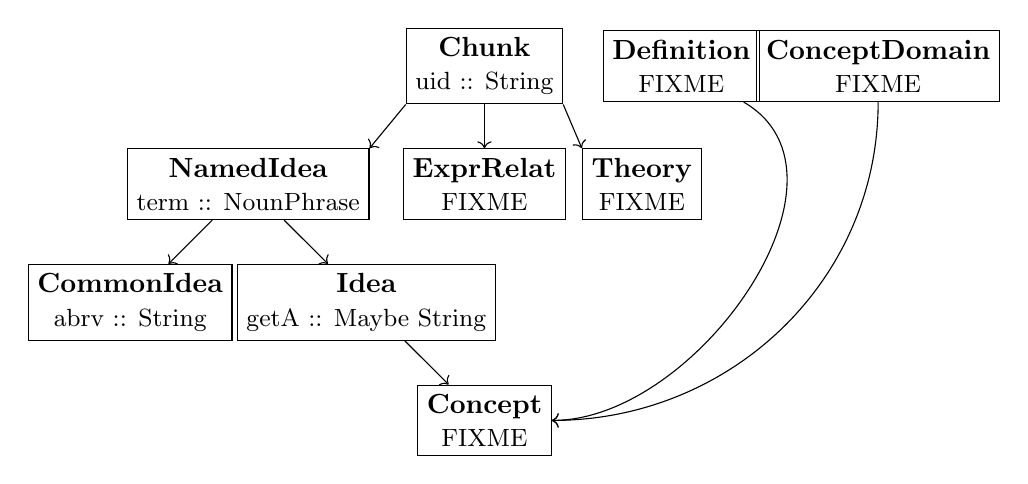
\begin{tikzpicture}
[every text node part/.style={align=center}]
\begin{scope}[every node/.style={rectangle,draw}]

\node(Chunk) at (0,0) 
{\textbf{Chunk} \\ \small{uid :: String}};

    \node(NamedIdea) at (-3,-1.5) 
    {\textbf{NamedIdea} \\ \small{term :: NounPhrase}};

        \node(Idea) at (-1.5, -3)
		{\textbf{Idea} \\ \small{getA :: Maybe String}};

			\node(Concept) at (0, -4.5)
			{\textbf{Concept} \\ \small{FIXME}};

        \node(CommonIdea) at (-4.5, -3)
        {\textbf{CommonIdea} \\ \small{abrv :: String}};

	\node(ExprRelat) at (0, -1.5)
	{\textbf{ExprRelat} \\ \small{FIXME}};

	\node(Theory) at (2, -1.5)
	{\textbf{Theory} \\ \small{FIXME}};

\node(Definition) at (2.5, 0)
{\textbf{Definition} \\ \small{FIXME}};

\node(ConceptDomain) at (5,0)
{\textbf{ConceptDomain} \\ \small{FIXME}};

%TODO: Finish and make this look nice

\end{scope}

\draw [->] (Chunk.south west) -- (NamedIdea.north east);
\draw [->] (Chunk.south) -- (ExprRelat.north);
\draw [->] (Chunk.south east) -- (Theory.north west);
\draw (NamedIdea) [->] to (CommonIdea);
\draw (NamedIdea) [->] to (Idea);
\draw (Definition) [->, out=330, in=0] to (Concept);
\draw (ConceptDomain) [->, out=270, in=0] to (Concept);
\draw (Idea) [->] to (Concept);

\end{tikzpicture}

%\begin{forest}
%  for tree={
%    align=center,
%    parent anchor=south,
%    child anchor=north,
%    font=\sffamily,
%    edge={thick, -{Stealth[]}},
%    l sep+=10pt,
%    edge path={
%      \noexpand\path [draw, \forestoption{edge}] (!u.parent anchor) -- 
%      +(0,-10pt) -| (.child anchor)\forestoption{edge label};
%    }
%  }
%  [\textbf{Chunk} \\ \small{uid :: String}
%    [\textbf{NamedIdea} \\ \small{term :: NounPhrase}
%      [\textbf{Idea} \\ \small{getA :: Maybe String}]
%      [\textbf{CommonIdea} \\ \small{abrv :: String}]
%    ]
%    [\textbf{Theory} \\ \small{FIXME}]
%    [\textbf{ExprRelat} \\ \small{FIXME}]
%  ]
%  [\textbf{Definition} \\ \small{uid :: String}
%  ]
%\end{forest}
\caption{Chunk hierarchy in Drasil Today}
\label{Fig:ChunkHierarchy}
\end{figure}

- We have to capture all of the information surrounding a piece of 
	knowledge to create our artifacts, regardless of whether that information 
	is relevant to any one particular artifact.
- Once knowledge is properly captured, we shouldn't have to capture it again if 
we want to reuse it in a different project.

\subsection{(Re-)Using Knowledge}

- Most obvious benefit -> no more copy/paste! Just reuse the chunk you need.
- Transformations
  - Represent different 'views' of the knowledge based on how abstract, what
    audience, etc.
    - Translate the knowledge into its requisite form (eqns, descriptions, code)
    - Variabilities -> different projects in the same family.
      - Easy to specialize to different family members
      - Example: SWHS vs NoPCM
      \fgr{} Show portion of each SRS, one similarity, one difference?
- Requires a framework / tool support to automate rendering of these 
transformations, otherwise it is even more work for humans.

\section{Drasil}
\label{S:Drasil}
- To use KBSE to its potential we need a strong support framework
- Intro to Drasil
    \fgr{} Knowledge tree
  - What it is and does
    - Domain Specific Language
    - Generate all the things!
  - Dev to date.
  - How is Knowledge Capture handled in Drasil? - chunks!
  - What do transformations look like? Recipes!
    \fgr{} SmithEtAl template for SRS = Drasil.DocumentLanguage
  - Key components of the generator / renderer

\subsection{Developing Drasil - A grounded theory} %DS Should this be here or 
													%in bg?
- Following grounded theory (ish). Using data from case studies to guide 
development and implement new features.
- \fgr{}: Before and after System Information.
- \fgr{}: Before and after mini-DBs
- Majority of features developed after analyzing commonalities in the case 
studies and abstracting them out.
- Allows for rapid progress -> constant iteration based on what we find in the 
data.

\subsection{Drasil Today}

- Sentence and Document
- Explain the chunk hierarchy (refer to Section~\ref{S:KnowCapt} figure)
- Data.Drasil
  \fgr{} Knowledge areas we've started to capture (See: SE-CSE paper)
- Recipe Language(s) -- Refer to:
  \fgr{} Drasil.DocumentLanguage
- The generator
  - HTML and TeX rendering
  - GOOL for code
- System Information -> Get into it

\section{Case studies - in more depth}

- Re-introduce case studies
  - Our methods for reimplementing
  - CI for testing
- Start showing off re-use and automated generation.
  - Start with common knowledge (generalized \fgr{}?)
  - Then onto GlassBR example to show off the doc lang recipe (\fgr{}?)
  - Then let's see SRS vs. NoPCM for reuse (particularly NoPCM) (\fgr{}?)


\subsection{Data.Drasil}

- Common knowledge
  \fgr{} SI\_Units
  \fgr{} Thermodynamics (ConsThermE?)

\subsection{GlassBR}

- Brief intro to problem GlassBR is solving - how it works
- Show off the doc language here
  \fgr{} GlassBR SRS in (truncated) DocLang format 
  - "Reads like a table of contents, with a few quirks"
- Show off some code generation
  \fgr{} Side-by-side of Chunk Eqn vs. Doc Eqn vs. Code 
  - "Easy to see that the code matches the equations"
- Talk about potential variabilities and how to make this a family
- Why is this interesting?
	- Fairly straightforward example of something a scientist would create/use 
	in their research

\subsection{NoPCM \& SWHS}

- Re-introduce the problems
- See how they're a family?
- Really drill in the similarities
  \fgr{} Figure showing NoPCM import(s)
- Lots of knowledge-reuse
- Very few 'new' chunks (count them?)
- Show example of variability in action
  \fgr{} Equation with/without PCM (rendered?)
- Why this example is interesting:
  - ODE solver -> We don't gen, just link to existing good one(s)

\subsection{Others}

- Mention SSP, Tiny, GamePhysics, but don't go too in-depth.
  - Useful examples as they give us a wider range of problems for analysis
- Testing
  - Physics is physics -> when we make updates, the underlying knowledge isn't
    changing, so neither should our output
  - Refer to CI

\subsection{Freebies - Compliments of System Information}

- Thanks to the recipe language and the way we structure out system information
  we can get
- Table of Symbols
- Table of Units
- Table of Abbreviations and Acronyms
- Bibliography

- All tedious to do by hand, but are free to automatically generate
- Generator includes sanity-checking -> Can't use something that isn't defined!
- Sanity-checks are 'free' -> we can check for errors with our symbols,
  ensure units are consistent, guard against constraints, and ensure we only
  reference those things which are defined in our system. 
- Sanity-checks are run every time artifacts are generated.

\subsection{Results}

- Here we discuss the results we've seen so far.
- Had some of these case studies attempted to be certified, they would (should) 
have failed.
	- A number of common problems.

\subsection{Common issues across case studies}

- A number of undefined symbols even after multiple passes by humans. 
(Auto-generating the symbol table and including sanity-checking revealed them)

\subsection{NoPCM and SWHS}

- Along with the common errors, there was some sharing of PCM-related knowledge
  - Found because PCM symbols were not in the ToS and the sanity-check caught 
  it.
  - No way to specifically exclude knowledge that shouldn't 'exist' in a project
- Work in Kolmogorov complexity / MDL for NoPCM + SWHS?
- Kolmogorov/MDL implies less writing for the same artifacts -> less to sift 
through = maybe better?

\subsection{SSP}

- Symbols for given quantities changed throughout the documentation
  - Went unnoticed by a human for years! Found almost instantly by Drasil
    - the new symbols were undefined.

\subsection{Pervasive Bugs}

- Mistakes in knowledge can be found in all artifacts - more likely to be 
caught!
- Easy to track down errors (smart error messages point to the exact chunk 
causing the problem).

\section{Future Work}

[*SS* - Once we are capable of true variability in the documentation, we can
really start asking the question about what is the "best" documentation for a
given context.  In the future experiments could be done with presenting the same
information in different ways to find which approach is the most effective.]

[*SS* - Related to the previous point, the act of formalizing the knowledge that
goes into the requirements documentation forces us to deeply understand the
distinctions between difference concepts, like scope, goal, theory, assumption,
simplification, etc.  With this knowledge we can improve the focus and
effectiveness of existing templates, and existing requirements solicitation and
analysis efforts.  Teaching it to a computer.]

- Run an experiment to determine how easy it is to create new software with 
Drasil.

- Run an experiment to see how easy it is to find and remove errors with Drasil

- Experiment to see time saved in maintenance while using Drasil vs. not

\section{Conclusion}

- Easier to find errors (anecdotally) - future work will tell us if this holds.

\bibliography{drasil}
\bibliographystyle{acm}
\end{document}
